\normaltrue \difficilefalse \tdifficilefalse
\correctiontrue
%\UPSTIidClasse{11} % 11 sup, 12 spé
\newcommand{\UPSTIidClasse}{12}

\exer{Pompe à piston radial  $\star$ \label{C2:06:10}}
\setcounter{numques}{0}
\UPSTIcompetence[2]{C2-06}
\index{Compétence C2-06}
\index{Pompe à palettes}
\ifcorrection
\else
\textbf{Pas de corrigé pour cet exercice.}
\fi

\ifprof
\else
Soit le mécanisme suivant. On a $\vect{AO}=e\vect{i_0}$ et $\vect{AB}=\lambda(t)\vect{i_1}$. De plus $e=\SI{10}{mm}$ et $R=\SI{20}{mm}$. Le contact entre \textbf{0} et \textbf{2} en $B$ est maintenu en permanence (notamment par effet centrifuge lors de la rotation de la pompe).
\begin{center}
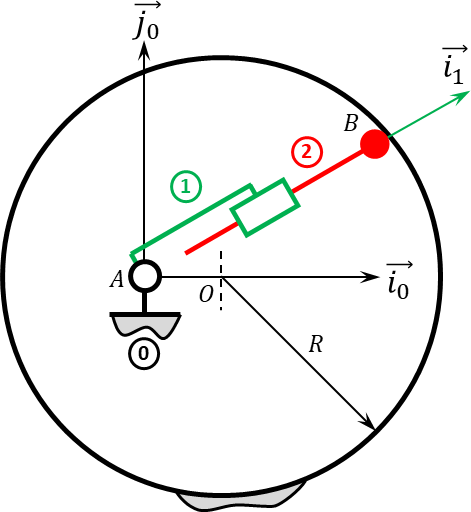
\includegraphics[width=\linewidth]{10_01}
\end{center}
\fi


\question{Tracer le graphe des liaisons.}

\ifprof
\begin{center}
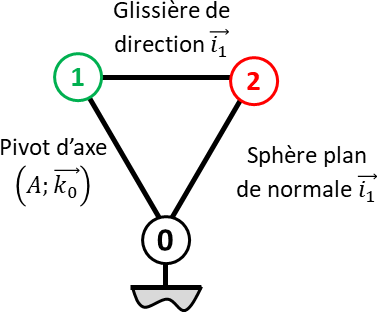
\includegraphics[width=.3\linewidth]{10_01_c}
\end{center}
\else
\fi

\question{Exprimer $\lambda(t)$ en fonction de $\theta(t)$.}

\ifprof
On a $\vect{OA}+\vect{AB}+\vect{BO}=\vect{0}$
soit $-e\vi{0}+\lambda\vi{1}-R\vect{u}=\vect{0}$
$\Leftrightarrow -e\vi{0}+\lambda(t)\cos\theta(t)\vi{0}+\lambda(t)\sin\theta(t)\vj{0}-R\cos\varphi(t)\vi{0}-R\sin\varphi(t)\vj{0} = \vect{0}$.

En projetant les expressions sur $\vi{0}$ et $\vj{0}$, on a :
$\left\{
\begin{array}{l}
-e+\lambda(t)\cos\theta(t)-R\cos\varphi(t) = 0 \\
\lambda(t)\sin\theta(t)-R\sin\varphi(t) = 0 \\
\end{array}\right.
$

On cherche à supprimer $\varphi(t)$; donc 

$\left\{
\begin{array}{l}
-e+\lambda(t)\cos\theta(t)=R\cos\varphi(t)  \\
\lambda(t)\sin\theta(t)  = R\sin\varphi(t) \\
\end{array}\right.
$.

En élevant au carré les expressions et en sommant, on obtient 
$R^2 =\left(-e+\lambda(t)\cos\theta(t)\right)^2+\lambda(t)^2\sin^2\theta(t)$
$\Rightarrow R^2 =\left(-e+\lambda(t)\cos\theta(t)\right)^2+\lambda(t)^2\sin^2\theta(t)$

$\Rightarrow R^2 =e^2 -2e\lambda(t)\cos\theta(t)+\lambda(t)^2$.

Résolution de l'équation :
$\lambda(t)^2-2e\lambda(t)\cos\theta(t)+e^2 -R^2=0$.

On  a $\Delta = \left(-2e\cos\theta(t)\right)^2-4\left(e^2 -R^2\right)$
$ =4e^2\cos^2\theta(t)-4e^2+4R^2$.

On a donc 

$ \lambda(t)= \dfrac{2e\cos\theta(t)\pm \sqrt{4e^2\cos^2\theta(t)-4e^2+4R^2}}{2}$

$  =e\cos\theta(t)\pm \sqrt{e^2\cos^2\theta(t)-e^2+R^2}$
\else
\fi

\question{En utilisant Python, tracer ${\lambda}(t)$ en fonction de ${\theta}(t)$.}
\ifprof
On garde la solution positive et obtient la courbe suivante.

\begin{center}
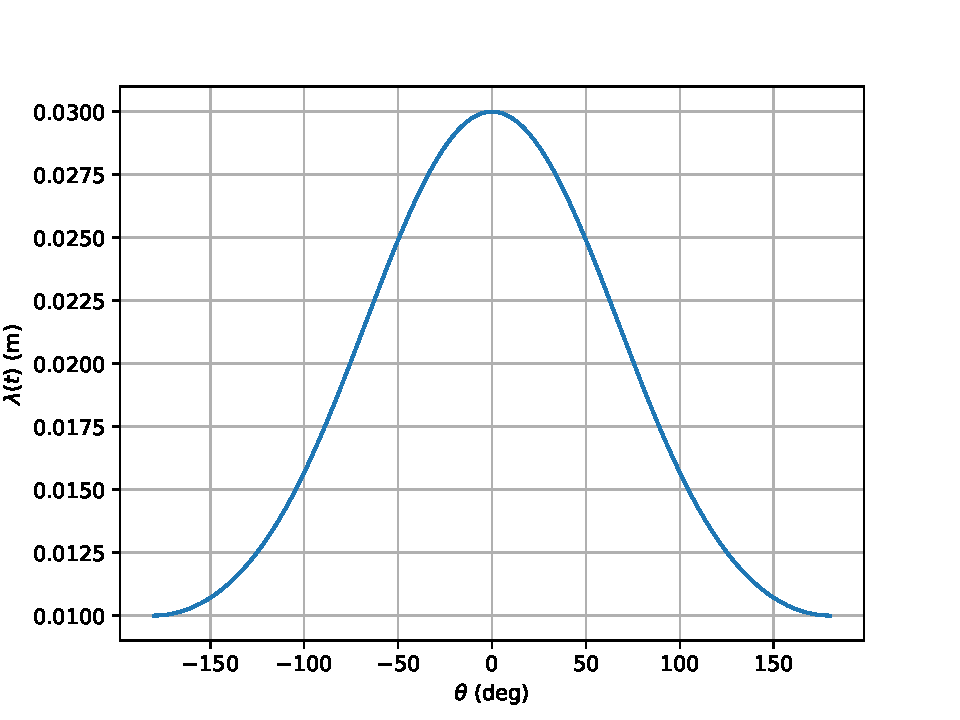
\includegraphics[width=.5\linewidth]{10_02_c}
\end{center}

\else
\fi

\question{Exprimer $\dot{\lambda}(t)$ en fonction de $\dot{\theta}(t)$.}

\ifprof

En dérivant l'expression précédente, on a 
$ \dot{\lambda}_{+}(t)= -e\dot{\theta}(t)\sin\theta(t)+  \dfrac{1}{2}\left( e^2\cos^2\theta(t)\right)'\left( e^2\cos^2\theta(t)-e^2+R^2\right)^{-\dfrac{1}{2}} $

$= -e\dot{\theta}(t)\sin\theta(t)-  \dfrac{ e^2\dot{\theta}(t)\cos\theta(t)\sin\theta(t)}{ \sqrt{e^2\cos^2\theta(t)-e^2+R^2}}$.

 \textbf{À revoir}
\begin{center}
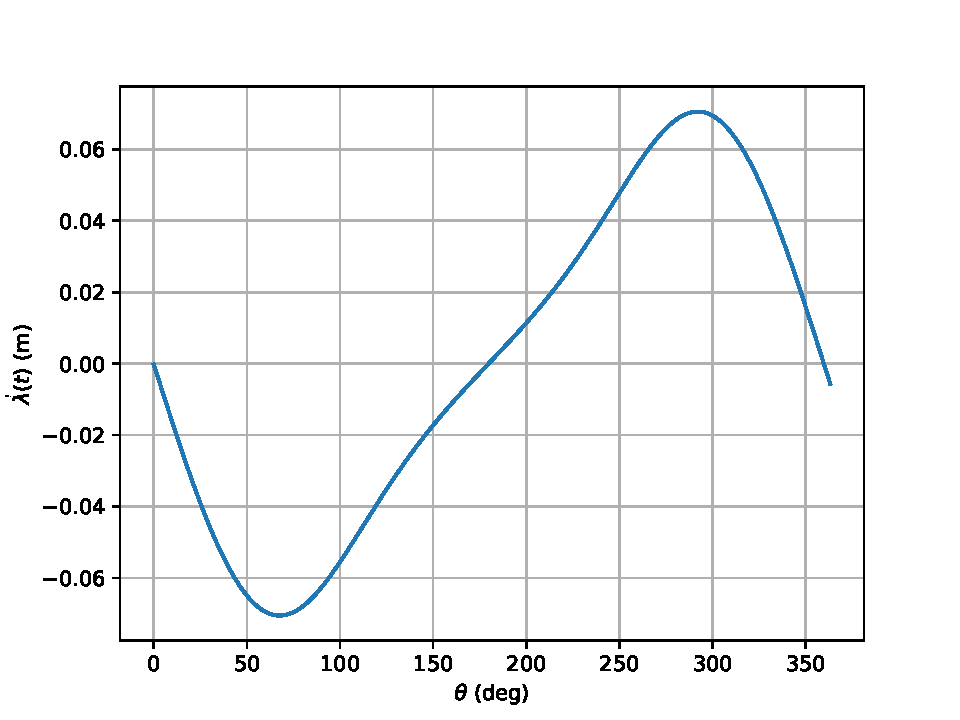
\includegraphics[width=.5\linewidth]{10_03_c}
\end{center}

\else
\fi

\ifprof
\else
On prendra une section de piston \textbf{2} de $\SI{1}{cm^2}$ et une fréquence de rotation de $\dot{\theta}(t)=\SI{2\pi}{rad.s^{-1}}$.
\fi
\question{Exprimer le débit instantané de la pompe.}

\ifprof
Le débit instantané de la pompe est donné par $q(t)=S\dot{\lambda}(t)$.
\else
\fi

\question{En utilisant Python, tracer le débit instantané de la pompe pour un tour de pompe pour $e=\SI{10}{mm}$ et $e=\SI{15}{mm}$.}


\ifprof
\begin{center}
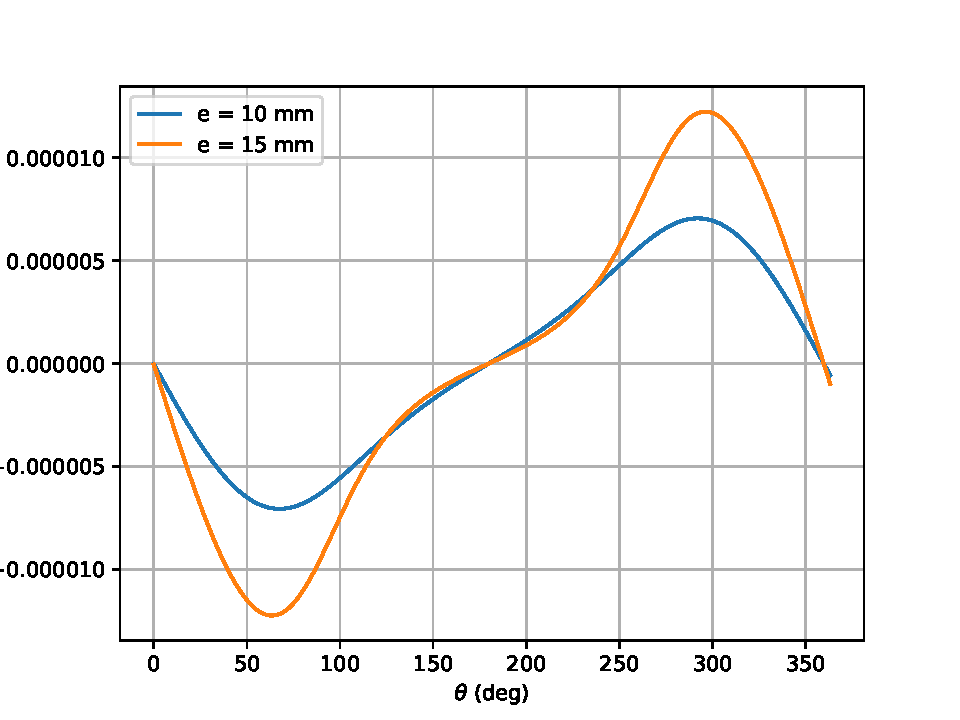
\includegraphics[width=.5\linewidth]{10_04_c}
\end{center}
\else
\fi

\question{En utilisant Python, tracer le débit instantané de la pompe pour un tour de pompe pour $e=\SI{10}{mm}$ pour une pompe à 5 pistons (5 branches \textbf{1+2}). }
\ifprof
\begin{lstlisting}
def plot_debit5p():
    plt.cla()
    w = 2*m.pi # rad/s (1tr/s)
    les_t = np.linspace(0,6,6000)
    les_theta = w*les_t
   
    # Calcul de la vitesse instantanée des pistons.
    les_lambda = calc_lambda(les_theta)
    les_lambdap = calc_lambdap_bis(les_t,les_lambda)
    les_lambdap = np.array(les_lambdap)
    
    S= 1e-4 # Surface en m2
    
    # 5 courbes de débit décalées d'un cinquième de tour
    les_q1 = S*les_lambdap
    les_q2 = S*les_lambdap[200:]
    les_q3 = S*les_lambdap[400:]
    les_q4 = S*les_lambdap[600:]
    les_q5 = S*les_lambdap[800:]
    
    # On conserve que les valeurs que sur un tour
    les_q1 = les_q1[:1000]
    les_q2 = les_q2[:1000]
    les_q3 = les_q3[:1000]
    les_q4 = les_q4[:1000]
    les_q5 = les_q5[:1000]
    plt.grid()
    
    les_t = les_t[:1000]
    les_theta = les_theta[:1000]
  
    plt.xlabel("$\\theta$ (deg)")
    plt.ylabel("Débit instantané $m^3s^{-1}$")
    
    # On conserve que les valeurs positives (débit)
    for i in range(len(les_q1)):
        if les_q1[i]<0:
            les_q1[i]=0
        if les_q2[i]<0:
            les_q2[i]=0
        if les_q3[i]<0:
            les_q3[i]=0
        if les_q4[i]<0:
            les_q4[i]=0
        if les_q5[i]<0:
            les_q5[i]=0

    plt.plot(np.degrees(les_theta),les_q1)
    plt.plot(np.degrees(les_theta),les_q2)
    plt.plot(np.degrees(les_theta),les_q3)
    plt.plot(np.degrees(les_theta),les_q4)
    plt.plot(np.degrees(les_theta),les_q5)
    
    # Le débit instantané est la sommme des contributions
    plt.plot(np.degrees(les_theta),les_q1+les_q2+les_q3+les_q4+les_q5)
    #plt.show() 
    #plt.savefig("10_05_c.pdf")
\end{lstlisting}

\begin{center}
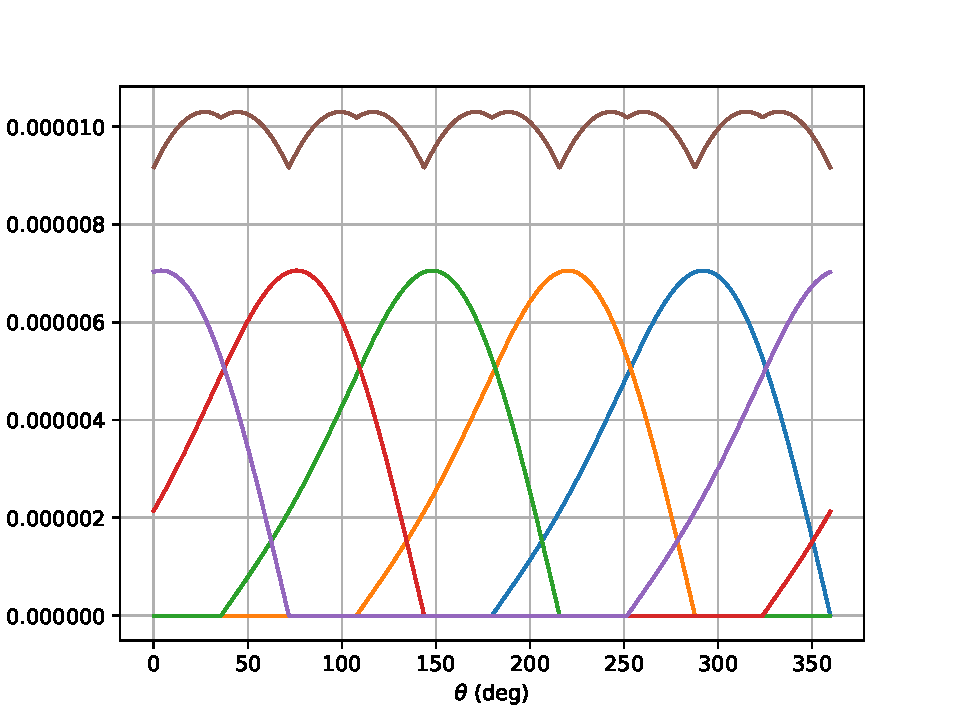
\includegraphics[width=.5\linewidth]{10_05_c}
\end{center}
\else
\fi


\ifprof
\else
\footnotesize
\begin{center}
\begin{tabular}{|p{.9\linewidth}|}
\hline
Indications :
\begin{enumerate}
\item .
\item $ \lambda(t)= e\cos\theta(t)\pm \sqrt{e^2\cos^2\theta(t)-e^2+R^2}$.
\item .
\item $q(t)=S\dot{\lambda}(t)$.
\item .
\end{enumerate} \\ \hline
\end{tabular}
\end{center}
\normalsize
\begin{flushright}
\footnotesize{Corrigé  voir \ref{C2:06:10}.}
\end{flushright}%
\fi